\chapter{Componenti di un sistema operativo}
\label{chap:componentiSO}

Dopo aver definito cosa sia un sistema operativo, vediamo ora quali siano le sue componenti principali, a partire dalla gestione dei processi e della memoria (primaria e secondaria), per poi passare alla gestione dei dell \texttt{I/O} e dei file fino ad arrivare alla protezione, la gestione della rete e l'interprete dei comandi.

\section{Le Componenti in generale}

    \subsubsection{Gestione dei Processi}
        \begin{definition}[Processo]
            Un \textbf{processo} è un programma in esecuzione che necessita di \textbf{risorse} per poter funzionare. Questo inoltre è eseguito in modo \textbf{sequenziale} ed \textbf{una istruzione alla volta}, infine è possibile che un processo sia del \texttt{SO} o dell'utente.
        \end{definition}
        In materia di gestione dei processi il sistema operativo è responsabile nella loro creazione e distruzione, nella loro sospensione e ripresa e deve fornire dei meccanismi per la sincronizzazione e la comunicazione tra i processi stessi.

    \subsubsection{Gestione della memoria primaria}
        \begin{definition}[Memoria primaria]
            La \textbf{memoria primaria} è la memoria principale del computer che conserva dati condivisi dalla \texttt{CPU} e dai dispositivi \texttt{I/O} questa è direttamente accessibile dalla \texttt{CPU}, per essere eseguito un programma deve essere caricato in memoria.
        \end{definition}
        La gestione della memoria primaria richiede la gestione dello spazi di memoria oltre alla decisione su quale processo debba essere caricato in memoria e quale debba essere rimosso. Inoltre il sistema operativo deve fornire dei meccanismi allocare e de-allocare la memoria.

    \subsubsection{Gestione della memoria secondaria}
        \begin{definition}[Memoria secondaria]
            La \textbf{memoria secondaria} è una memoria \textbf{non volatile} ed \textbf{grande} rispetto alla memoria primaria, questa è utilizzata per memorizzare i dati e i programmi in modo \textbf{permanente}.
        \end{definition}
        Questa memoria consiste di uno o più dischi (magnetici) ed il sistema operativo deve fornire dei meccanismi per la gestione dello spazio libero, l'allocazione dello spazio ed lo \textit{scheduling} degli accessi ai dischi.

    \subsubsection{Gestione dell'\texttt{I/O}}
        Il \texttt{SO} nasconde la complessità dell'\texttt{I/O} ai programmi utente, fornendo un'astrazione dell'\texttt{I/O} e fornendo dei meccanismi per: accumulare gli accessi ai dispositivi (\textit{buffering}), fornire una interfaccia generica per i dispositivi e fornire dei \textit{driver} specifici (scritti in \texttt{C}, \texttt{C++} o \textit{assembly}). 

    \subsubsection{Gestione dei file}
        \begin{definition}[File]
            Un \textbf{file} è una sequenza di \textit{byte} memorizzata in un qualsiasi supporto fisico controllato da \textit{driver} del sistema operativo.
        \end{definition}
        Un file è dunque un'astrazione logica per rendere più semplice la memorizzazione e l'uso della memoria \textbf{non volatile}. Il sistema operativo deve fornire dei meccanismi per la creazione, la cancellazione, la lettura e la scrittura di file e \textit{directory} oltre a fornire delle primitive (copia, sposta, rinomina) per la gestione dei file. 

    \subsubsection{Protezione}
        Il sistema operativo deve fornire dei meccanismi per controllare l'accesso a tutte le risorse da parte di processi e utenti, inoltre l'\texttt{SO} è responsabile della definizione di accessi autorizzati e non autorizzati, oltre a definire i controlli necessari ed a fornire dei meccanismi per verificare le politiche di accesso definite.

\section{Come usare i servizi dei sistemi operativi}
    Il sistema operativo metta a disposizione le sue interface tramite delle \textit{system call} che sono delle chiamate a funzione che permettono di accedere ai servizi del sistema operativo precedentemente descritti. Queste chiamate a funzione sono utilizzate per eseguire operazioni che richiedono privilegi di sistema, come ad esempio la gestione dei processi, della memoria, dell'\texttt{I/O} e dei file.
    \subsection{Interprete dei comandi}
        Un esempio di utilizzo delle \textit{system call} è l'interazione con l'interprete dei comandi, che permette di eseguire comandi e programmi tramite una interfaccia testuale. Questo interprete tramuta i comandi in \textit{system call} che vengono poi eseguite dal sistema operativo. Questo permette di creare e gestire processi, gestire \texttt{I/O}, disco, memoria e file oltre alla gestione delle protezione e della rete.\newline
        Nel \texttt{SO} esistono dei comandi predefiniti che possono essere chiamati direttamente per il loro nome, questi sono implementati con una semantica specifica e possono essere utilizzati per eseguire operazioni di base, nel caso di comandi non predefiniti è possibile scrivere dei programmi che vengono eseguiti dall'interprete dei comandi.
    
    \subsection{L'interfaccia grafica}
        Un'altra interfaccia che permette di interagire con il sistema operativo è l'interfaccia grafica, che permette di interagire con il sistema operativo tramite il \textit{mouse} e la tastiera. Questa interfaccia più intuitiva e facile da usare rispetto all'interprete dei comandi, permette di interagire con il \texttt{SO} tramite icone e finestre. Questa interfaccia, anche se più semplice, non è per forza più veloce dell'interprete dei comandi, in quanto l'interfaccia grafica è più lenta e richiede più risorse rispetto all'interprete dei comandi.

    \subsection{\textit{System calls}}
        I processi non usano le \textit{shell} per eseguire le \textit{system call}, ma usano delle \texttt{API} (\textit{Application Programming Interface}) che permettono di accedere ai servizi del sistema operativo. Queste \texttt{API} sono delle librerie di funzioni ad alto livello che permettono di accedere ai servizi del sistema operativo. Queste librerie sono scritte in \texttt{C} o \texttt{C++} e permettono di accedere ai servizi del sistema operativo in modo più semplice e più sicuro rispetto all'uso diretto delle \textit{system call}.
        \paragraph{Esempio di \texttt{API}} Un esempio di \texttt{API} è la \texttt{Win32}, prendiamo in esame la funzione \texttt{ReadFile} che permette di leggere un file:
\begin{lstlisting}[language=C]
    BOOL ReadFile (
        HANDLE file,
        LPVOID buffer,
        DWORD bytes to read,
        LPDWORD bytes read,
        LPOVERLAPPED ovl
    );
\end{lstlisting}
        Questa funzione ritorna un valore booleano che indica se la funzione è andata a buon fine o meno, inoltre questa funzione prende in input il file da leggere, il buffer in cui scrivere i dati letti, il numero di byte da leggere, il numero di byte letti e un puntatore a una struttura \texttt{OVERLAPPED} che permette di specificare un offset per la lettura.
        \subsubsection{Le \texttt{API} nei diversi \texttt{SO}}
            Le 2 \texttt{API} più comuni per Windows sono: \texttt{Win32} e \texttt{Win64} mentre per Linux sono: \texttt{POSIX} (\textit{Portable Operating-System Interface}) che includono le \textit{system call} per tutte le versioni di \texttt{UNIX}, \textit{Linux} e \textit{Mac OS X}, o tutte le distribuzioni \texttt{POSIX}\textit{-compliant}. 
            \paragraph{\textit{Windows} su \textit{Linux}} Per eseguire programmi \textit{Windows} su \textit{Linux} è possibile usare \texttt{Wine} che è un \textit{emulatore} il quale traduce le chiamate \texttt{API} di \textit{Windows} in chiamate \texttt{API} di \textit{Linux} \textit{on-the-fly}, ovvero durante l'esecuzione del programma. Questo permette di eseguire programmi \textit{Windows} su \textit{Linux} senza dover riscrivere il codice del programma.
        
        \subsubsection{Implementazione delle \textit{System Call}}
            Ad ogni \textit{system call} è associato un numero univoco, che permette al sistema operativo di identificare la \textit{system call} richiesta. È compito dell'interfaccia tenere traccia dei numeri associati alle \textit{system call} e di passare i parametri alla \textit{system call} richiesta. Questa interfaccia invoca la \textit{system call} nel \textit{kernel} del sistema operativo, che esegue la \textit{system call} e ritorna il risultato al chiamante. Questo meccanismo permette al chiamante di non dover conoscere i dettagli di implementazione della \textit{system call} ma solo la sua interfaccia.
            \paragraph{Esecuzione delle \textit{system calls}} Per eseguire una \textit{system call} dopo che il processo ha eseguito la chiamata all'interfaccia del \texttt{SO} il quale conoscendo il numero della \textit{system call} controlla dove questa è implementata tramite la \textit{system call table} (una tabella che contiene i puntatori alla implementazione delle \textit{system call}). Una volta trovata la \textit{system call} il \texttt{SO} esegue la \textit{system call} e ritorna il risultato al chiamante.
            \paragraph{Opzioni per il passaggio dei parametri} I parametri di una \textit{system call} possono essere passati in diversi modi. I più comuni sono: passaggio tramite registri, passaggio tramite lo \texttt{stack} e passaggio tramite puntatori. Il passaggio tramite registri è il più veloce ma permette di passare pochi parametri e di piccola dimensione, il passaggio tramite lo \texttt{stack} permette di passare più parametri e di dimensioni maggiori, infine il passaggio tramite puntatori permette di passare parametri di dimensioni maggiori e di passare parametri complessi, ma và passata una tabella di parametri che deve essete passata tramite \texttt{stack} o registri.
                \subparagraph{Parametri tramite \texttt{stack}} Il passaggio dei parametri tramite \texttt{stack} avviene in questo modo:
                    \begin{enumerate}
                        \item[1-3] Salvataggio parametri sullo \texttt{stack}
                        \item[4] Chiamata della funzione di libreria
                        \item[5] Caricamento del numero della \textit{system call} su un registro \texttt{Rx}
                        \item[6] Esecuzione \texttt{TRAP} (Passaggio in \textit{kernel mode})
                        \item[7-8] Esecuzione della \textit{system call}
                        \item[9] Ritorno al chiamante 
                        \item[10-11] Ritorno al codice utente ed incremento dello \texttt{stack pointer} 
                    \end{enumerate}
                    \begin{figure}[H]
                        \centering
                        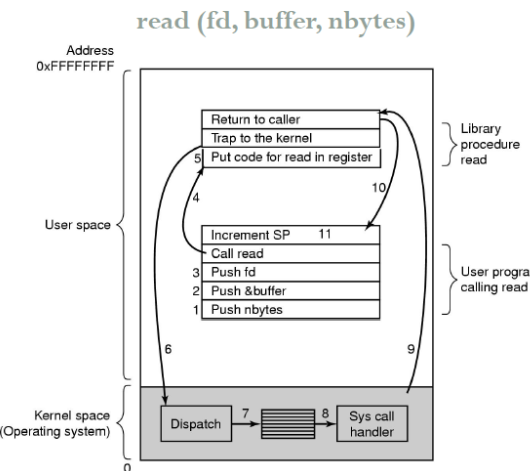
\includegraphics[width=0.3\textwidth]{images/02/stackCall.png}
                        \caption{Passaggio dei parametri tramite \texttt{stack}}
                    \end{figure}
                \subparagraph{Passaggio di parametri tramite tabella} 
                    Come anticipato il passaggio di parametri tramite tabella viene utilizzato per passare parametri complessi o di dimensioni maggiori andando a passare un puntatore alla tabella che contiene i parametri. Questo metodo permette di passare un numero maggiore di parametri e di dimensioni maggiori in quanto i parametri sono passati per riferimento alla memoria primaria.
                    \begin{figure}[H]
                        \centering
                        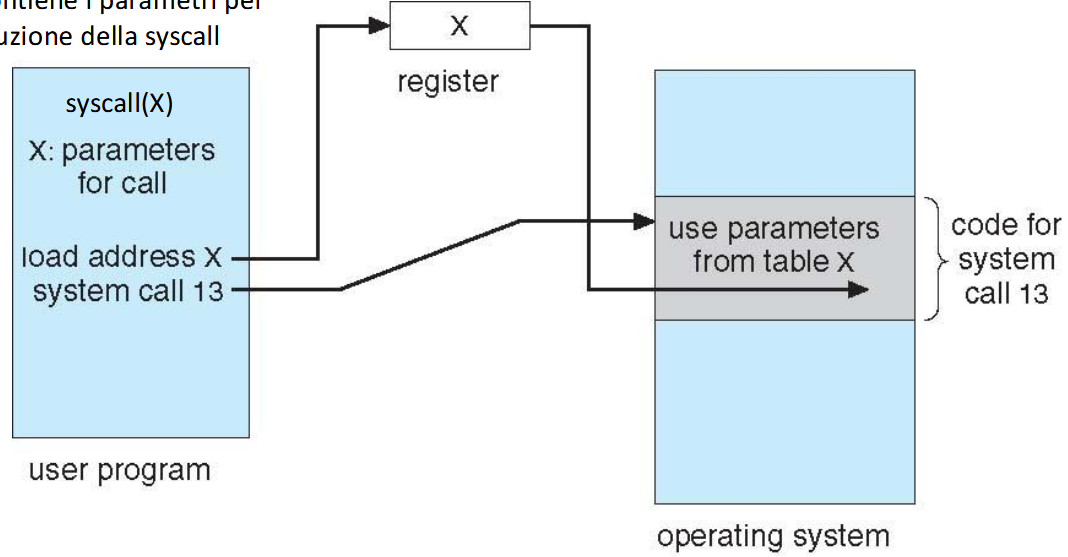
\includegraphics[width=0.3\textwidth]{images/02/tabCall.png}
                        \caption{Passaggio dei parametri tramite tabella}
                    \end{figure}
                    